\chapter{Numerical Simulation of a Baroclinic Life Cycle}
\label{ch:ch3}
\section{Analytic Initial Conditions for a Double Jet}
As outlined in Chapter \ref{ch:ch1}, baroclinic instabilities are of interest to researchers for many reasons; for example, the resulting weather patterns baroclinic wave life cycles give rise to. To study a jet in a channel, one of the common initialization techniques is to prescribe a small, zonally invariant potential vorticity (PV) in the troposphere combined with a larger (usually by an order of magnitude)  PV in the stratosphere (e.g.\  \cite{Zhang2004}, \cite{Plougonven2007}, \cite{Waite2009}).  To represent the tropopause, a function with a sharp gradient (e.g.\ hyperbolic tangent function) can be used to separate the troposphere and the tropopause. The initial velocity field can then be recovered by iteratively inverting the PV (e.g\ \cite{Plougonven2007}). Instead of this iterative procedure, it can be advantageous to have an analytic initial conditions for multiple reasons. For example, by referring to the vertical structure problem in Section \ref{sec:normalModes}, the derivative of the static stability can be analytically written, removing the error that would be introduced from a numerical computation. Additionally, parameters can be adjusted to allow for different initial conditions, such as including a $\beta$-plane or adding moisture.\\

 However, creating initial fields for an analytic jet is not a trivial task, as the jet must be a steady-state solution to the governing equations and must also contain strong vertical shear in order to create baroclinic instability in the atmosphere. It is for this reason that we take a modified approach to the jet in a channel presented in a 2015 paper by Ullrich, Reed, and Jablonowski (hereafter referred to as URJ15) \cite{Ullrich2015}. This jet is formulated to initially be in hydrostatic, geostrophic, and thermal wind balance in a 3-D channel. In addition, URJ15 develop the initial conditions in $\eta = p/p_0$ coordinates, consistent with the normal mode formulation of Chapter \ref{ch:ch2}. In this section, the setup of the (single) zonal jet in a 3-D channel by URJ15 is presented, as well as the modifications made to transform the jet into a double jet in a doubly-periodic domain.

\subsection{Velocity Field in a Channel}
The initial velocity field consists of a zonal wind given by 
\begin{align}
u(x,y,\eta) = -u_0 \sin^2 { \left(\frac{\pi y}{L_y}\right)} \ln{\eta} \exp{\left\{-\left(\frac{\ln \eta}{b}\right)^2\right\}}.
\end{align}
Here $u_0$, $L_y$, and $b$ are tunable physical parameters. Refer to Table \ref{tab:parameters} for specific parameters used in the simulations for this thesis. Note that the zonal velocity field is independent of $x$, as one would expect for a zonal jet.\\


The prescribed zonal velocity field has several desirable features. The meridional-varying part ensures the zonal velocity goes to 0 at the boundaries $y = 0, L_y$, while the pressure-dependent part ensures that the velocity approaches 0 at both the surface and model top. It can be shown that the velocity reaches a maximum value at around 240 hPa, which is close to the observations of mid-latitude jets \cite{Ullrich2015}. One important thing to note is that the parameter $u_0$ does not actually set the maximum velocity. In fact, the true maximum lies at a value slightly less than this parameter. \\

\begin{table}[H]
\centering
\begin{tabular}{|c|l|l|}
\hline
\textbf{Parameter} & \textbf{Description} & \textbf{Value} \\ \hline
$u_0$ & velocity scale factor for the jet & $55~\text{m s}^{-1}$ \\ \hline
$L_y$ & Channel width in meridional direction & $5120~\text{km}$ \\ \hline
$b$ & dimensionless vertical width parameter of jet & $ 2$ \\ \hline
$T_0$ & surface temperature & 288 K \\ \hline
$g$ & acceleration due to gravity &  $9.81~\text{m s}^{-1}$\\ \hline
$\Gamma$ & lapse rate & $0.005~\text{K m}^{-1}$\\ \hline
$R_d$ & ideal gas constant of dry air & $287 ~\text{J kg}^{-1} \text{K}^{-1}$ \\ \hline
$f_0$ & Coriolis parameter & $ 1.03 \times 10^{-4} ~\text{s}^{-1}$ \\ \hline
\end{tabular}
\caption{Parameters used in the initialization of the analytic jet.}
\label{tab:parameters}
\end{table}
The meridional velocity and vertical velocity are both set to 0 initially. From the initial velocity fields, it is trivially non-divergent (i.e.\ $\delta = 0$).\\

The vertical vorticity is likewise easy to compute, and can be represented by
\begin{align}
\zeta(x,y,\eta) = -\frac{\partial u}{\partial y} = \frac{2\pi u_0}{L_y} \sin{\left(\frac{\pi y}{L_y}\right)} \cos{\left(\frac{\pi y}{L_y}\right)} \ln{\eta} \exp{\left\{-\left(\frac{\ln \eta}{b}\right)^2\right\}}.
\end{align}

Figure \ref{fig:initialVelVort} shows a meridional-vertical cross section of the velocity and vertical vorticity fields of the jet.
\begin{figure}[H]
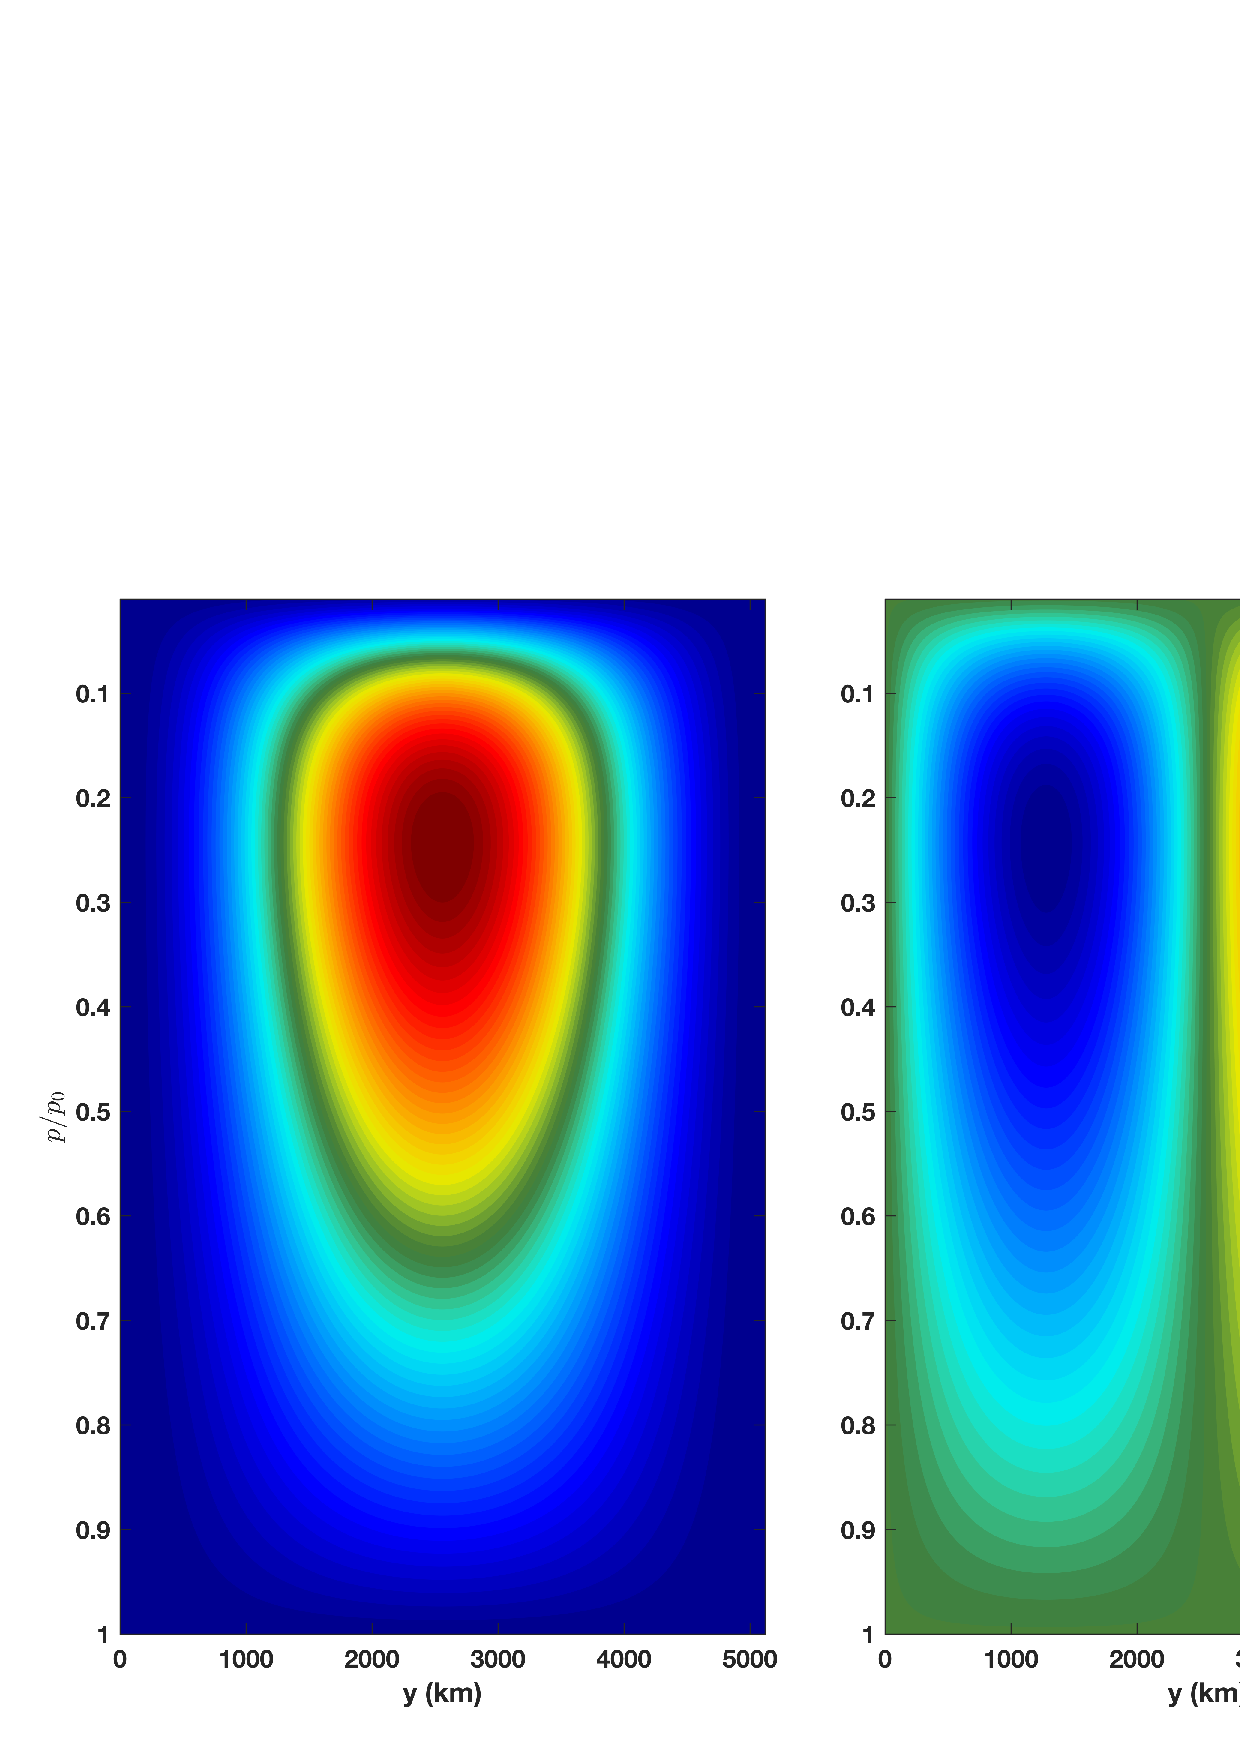
\includegraphics[scale=1]{Chapter3/img/initialVelVort}
\caption{Meridional slice of initial velocity (in m $\text{s}^{-1}$, top) and vertical vorticity (in $\text{s}^{-1}$, bottom) of the single jet.}
\label{fig:initialVelVort}
\end{figure}

\subsection{Geopotential and Temperature Fields in a Channel}

The geopotential field is prescribed by a horizontal-mean geopotential given by

\begin{align}
\left\langle\Phi(\eta)\right\rangle = \frac{T_0 g}{\Gamma}\left(1 - \eta^{\frac{R_d \Gamma}{g}}\right),
\end{align}

where $T_0$ is the surface temperature, $g$ is the acceleration due to gravity, $R_d$ is the ideal gas constant for dry air, and $\Gamma$ is the lapse rate of the atmosphere. Note that $\Gamma$ in this section is different from the static stability $\tilde{\Gamma}$ from Section \ref{sec:normalModes}. This is then combined with a spatially varying deviation of the geopotential from the horizontal mean in order to maintain geostrophic balance. The total geopotential, including the deviation from the horizontal-mean, on an $f$-plane is given by

\begin{align}
\Phi(x,y,\eta) =\left\langle\Phi(\eta)\right\rangle +  \Phi'(x,y)\ln{\eta} \exp{\left\{ -\left(\frac{\ln{\eta}}{b}\right)^2\right\}},
\end{align}
with $\Phi'(x,y)$ given by
\begin{align}
\Phi'(x,y) = \frac{u_0 f_0}{2}\left[y - \frac{L_y}{2} - \frac{L_y}{2\pi} \sin{\left(\frac{2\pi y}{L_y}\right)}\right] .
\end{align}
Here, $u_0$ is the same parameter as in the initial velocity field, and $f_0$ is the $f$-plane Coriolis paramter (approximately $10^{-4} ~\text{s}^{-1}$ at a latitude of $45\degree$). URJ15 provide a more complicated expression to allow for the possibility of a $\beta$-plane, but the normal mode theory from Chapter \ref{ch:ch2} focuses solely on the $f$-plane.\\

In addition to prescribing the velocity fields and geopotential field, a temperature field is required to completely describe the initial state of the jet. Similarly to the geopotential, the temperature field is composed of a horizontal-mean temperature field with a deviation from this base state. The horizontal-mean temperature is given by

\begin{align}
\left\langle T(\eta)\right\rangle = T_0 \eta^{\frac{R_d \Gamma}{g}}.
\end{align}

In order to be initially in hydrostatic balance, a deviation from the horizontal-mean temperature is given by

\begin{align}
T'(x,y,\eta) = \frac{\Phi'(x,y)}{R_d} \left\{ \frac{2}{b^2}(\ln {\eta})^2 - 1\right\} \exp{\left\{-\left(\frac{\ln{\eta}}{b}\right)^2\right\} }.
\end{align}

Figure \ref{fig:initialGeo} shows the initial geopotential field, while Figure \ref{fig:tempBuoy} shows the vertical profile of the stratification of the atmosphere proposed by URJ15. 

\begin{figure}[H]
\includegraphics[scale=1]{Chapter3/img/initialGeo}
\caption{Meridional slice of the geopotential field ($\text{m}^2~\text{s}^{-2}$) for a single jet.}
\label{fig:initialGeo}
\end{figure}

Although the initial conditions for the atmosphere proposed by URJ15 notably lack a tropopause, the atmosphere is still stably stratified and the sharp increase in Br{\"u}nt-Vaisala frequency near the domain top helps to further reduce gravity wave reflections off of the lid.

\begin{figure}[H]
\includegraphics[scale=1]{Chapter3/img/tempBuoy}
\caption{Initial mean vertical profile of the horizontal mean temperature (left) and Brunt-V\"ais\"al\"a frequency (right).}
\label{fig:tempBuoy}
\end{figure}



\subsection{Extension From a Channel to a Doubly-Periodic Domain}
To take advantage of the Fourier transform in the meridional direction without involving the complicated boundary conditions for the normal mode decomposition that arise from a channel, we extend the analytic formulas presented by URJ15 to doubly-periodic domain while maintaining an initially balanced system.\\

The domain is extended from $y \in [0, L_y]$ to $y \in [-L_y, L_y]$. The geopotential and temperature fields are chosen to be even extensions about $y=0$. This choice is physically sensible as it maintains hydrostatic balance.\\

For the velocity fields, the meridional and vertical fields are still chosen to be 0, but the zonal velocity field must be altered to maintain geostrophic balance. Since $\Phi$ was evenly extended about $y=0$, $\partial \Phi/\partial y$ is odd about $y = 0$. We therefore require that the zonal velocity field be an odd extension about $y = 0$. A meridional slice of the geopotential in Figure \ref{fig:initialGeoDouble} and the initial velocity and vertical vorticity fields in Figure \ref{fig:initialVelVortDouble} show the new extended doubly-periodic domain with a double jet.\\

\begin{figure}[H]
\includegraphics[scale=1]{Chapter3/img/initialGeoDouble}
\caption{Meridional slice of the initial geopotential ($\text{m}^2 ~\text{s}^{-2}$) after the domain has been extended to be doubly periodic.}
\label{fig:initialGeoDouble}
\end{figure}

\begin{figure}[H]
\includegraphics[scale=1]{Chapter3/img/initialVelVortDouble}
\caption{Meridional slice of initial velocity (top, in $\text{m s}^{-1}$) and vertical vorticity (bottom, in $\text{s}^{-1}$) after the domain has been extended to be doubly periodic.}
\label{fig:initialVelVortDouble}
\end{figure}
One final difference between the initial state presented in this thesis and in the initial state presented by URJ15 is the baroclinic wave triggering mechanism. URJ15 propose a Gaussian perturbation of the zonal velocity field. We choose to use a Gaussian perturbation of amplitude $4$ K  and root-mean-square width $600$ m to the potential temperature field, taking care to numerically recalculate the geopotential and density since the mass in the air column should not change, and we rebalance hydrostatically. Both approaches mean that the baroclinic jet is no longer in geostrophic balance, and high-speed gravity waves are triggered. URJ15 argue that the gravity waves are dampened by diffusion before the baroclinic life cycle begins, especially since the perturbation to the potential temperature field in our simulation is small.

\section{Model Choice and Simulation Overview}
\label{sec:simulationOverview}
To study the baroclinic life cycle, we employ the Weather Research and Forecasting model advanced research core (WRF-ARW) \cite{Skamarock2008}. WRF is a robust finite difference model with third order Runge-Kutta (RK3) time-split integration that solves the Euler equations. For the vertical coordinate, WRF uses a terrain-following, hydrostatic-pressure coordinate. It is non-hydrostatic, fully compressible, and the spatial discretization features $2^{nd}$ to $6^{th}$ order advection options. For this study, we use $5^{th}$ and $3^{rd}$ order horizontal and vertical advection, respectively. The odd-ordered schemes are upwind biased in WRF, adding numerical dissipation to the model. The WRF-ARW core is a parallelized model capable of running both real data simulations and idealized simulations. \\

Though WRF-ARW offers many physics options, including surface physics, cloud parameterizations, and microphysics, the work presented here is an idealized study. Therefore, the simulation is run without moisture, planetary boundary layer physics, surface physics, or radiation physics. No additional dissipation scheme is applied, as the numerical dissipation from the finite difference advection scheme does an adequate job of removing energy build up in the subgrid scale (discussed in Chapter \ref{ch:ch4}).\\

 The governing equations used by WRF are different from the linearized equations (\ref{eq:nmMomentum}-\ref{eq:nmThermo}) used to derive the normal mode theory. Though the model itself is non-hydrostatic, it uses a terrain-following pressure coordinate denoted by
\begin{align}
\eta = (p_h - p_{ht})/\mu \label{eq:wrfVert},
\end{align}
where $p_h$ is the hydrostatic pressure, $p_{ht}$ is the hydrostatic pressure at the model top, $\mu = p_{hs} - p_{ht}$ is the mass per unit area, and $p_{hs}$ is the hydrostatic pressure at the model surface. Note that this vertical coordinate is different from the $\eta$ coordinate used by URJ15. The dry WRF equations of motion following this pressure coordinate and written in flux-form are
\begin{align}
\frac{\partial U}{\partial t} + (\nabla \cdot \mathbf{V}u) - \frac{\partial p\Phi_eta}{\partial x} + \frac{\partial p\Phi_x}{\partial \eta} &= F_U,\label{eq:wrfXMomentum}\\
\frac{\partial V}{\partial t} + (\nabla \cdot \mathbf{V}v) - \frac{\partial p\Phi_eta}{\partial y} + \frac{\partial p\Phi_y}{\partial \eta} &= F_V, \label{eq:wrfYomentum}\\
\frac{\partial W}{\partial t} + (\nabla \cdot \mathbf{V}w) - g\left(\frac{\partial p}{\partial \eta} - \mu\right)& = F_W, \label{eq:wrfPMomentum}\\
\frac{\partial \Theta} {\partial t} + (\nabla \cdot \mathbf{V}\theta) &= F_\Theta, \label{eq:wrfThermo}\\
\frac{\partial \mu}{\partial t} + (\nabla \cdot \mathbf{V}) &= 0, \label{eq:wrfContinuity}\\
\frac{\partial \Phi}{\partial t} + \mu^{-1}\left[(\mathbf{V} \cdot \nabla \phi) - gW\right] &= 0, \label{eq:wrfGeopotential}
\end{align}
where $\mathbf{V} = \mu\mathbf{v}$, $\Theta = \mu\theta$, and $F_U$, $F_V$, $F_W$, and $F_\Theta$ represent the forcing terms from model physics, turbulent mixing, and Earth's rotation. Subscripts in equations (\ref{eq:wrfXMomentum} - \ref{eq:wrfYomentum}) represent partial derivatives. Equations (\ref{eq:wrfXMomentum} - \ref{eq:wrfContinuity}) are written in conservation form, while equation (\ref{eq:wrfGeopotential}) is not because $\mu\Phi$ is not a conserved quantity. For dry dynamics, the last thing WRF needs is a diagnostic equation for hydrostatic balance, given by
\begin{align}
\frac{\partial \Phi}{\partial \eta} + \frac{\mu}{\rho} = 0. \label{eq:wrfHydrostatic}
\end{align}
Note that the hydrostatic equation (\ref{eq:wrfHydrostatic}) does not constrain the solution, but instead is part of the vertical coordinate definition. The pressure, $p$, and hydrostatic pressure, $p_h$, are stored as two different state variables in the WRF model.\\

We use a moderate-resolution domain with a size of 1024x1024x100  points.  WRF uses an Arakawa C-grid \cite{Arakawa1977}, which staggers certain variables such as velocities to cell edges, while other variables such as geopotential, air mass columns, and potential temperature among others are kept at cell centers or ``mass points''. Refer to Figure \ref{fig:Cgrid} for an example layout of the Arakawa C-grid. This means that our zonal velocity field is actually $1025 \times 1024 \times 100$ points, the meridional velocity is $1024 \times 1025 \times 100$ points, and the vertical velocity its $1024 \times 1024 \times 101$ points. We use periodic boundary conditions in the horizontal. In the vertical, the free slip boundary condition is used at the bottom, while a constant pressure level at the top boundary along a material surface is combined with diffusive damping starting 5000 m from the top to reduce gravity wave reflections. \\
\begin{figure}[H]
\begin{center}
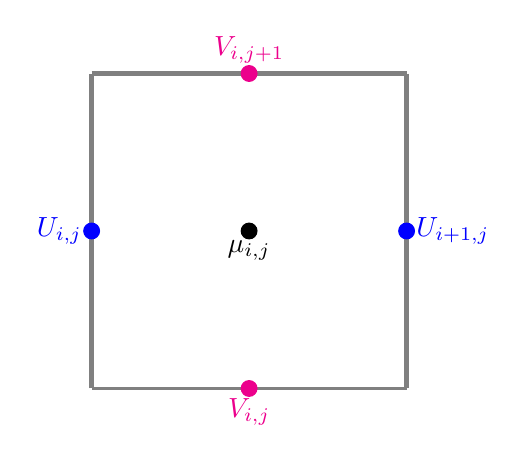
\begin{tikzpicture}
\draw[gray, ultra thick] (-2,-2) -- (-2,2);
\draw[gray, ultra thick] (-2,2) -- (2,2);
\draw[gray, ultra thick] (2,2) -- (2,-2);
\draw[gray, very thick] (2,-2) -- (-2,-2);

\filldraw[blue] (2,0) circle (0.1) node[anchor=west] {$U_{i+1,j}$};
\filldraw[blue] (-2,0) circle (0.1) node[anchor=east] {$U_{i,j}$};
\filldraw[magenta] (0,-2) circle (0.1) node[anchor=north] {$V_{i,j}$};
\filldraw[magenta] (0,2) circle (0.1) node[anchor=south] {$V_{i,j+1}$};
\filldraw[black] (0,0) circle (0.1) node[anchor=north] {$\mu_{i,j}$};
\end{tikzpicture}
\caption{An example of state variable positioning on a single cell in the Arakawa C-grid. This view is of a horizontal level (i.e.\ no vertical indices are shown, though vertical staggering is identical for the vertical velocity $w$). Here $A_{i,j}$ represents the $i^{th}$ row and the $j^{th}$ column of state variable $A$. Zonal and meridional velocities are staggered in the $x$- and $y$-directions, respectively. An example of a state variable stored at mass points is $\mu$, the mass per unit area in the air column.}
\label{fig:Cgrid}
\end{center}
\end{figure}

Our simulation uses a moderate resolution grid spacing of $\Delta x = \Delta y = 5~\text{km}$ in the horizontal, with $\Delta p \approx 10 ~\text{mbar}$ in the vertical. This corresponds to a domain size of $L_x = L_y = 5 120$ km in the horizontal and $L_z \approx 25$ km in the vertical. Since the grid is evenly spaced in $p$, the grid spacing in $z$ changes throughout the domain. $\Delta z$ near the surface is approximately $170$ m, while $\Delta z$ near the top is approximately $2000$ m. The time step is chosen to be $\Delta t = 30$ seconds for numerical stability reasons. The simulation is run for 15 days in model time, allowing sufficient time for the baroclinic instabilities to grow and saturate. During this time, a number of common mesoscale phenomena appear, such as surface fronts shown in Figure \ref{fig:frontSquall}. Kelvin-Helmholtz instabilities and PV spirals are commonly seen along these fronts \cite{Plougonven2013,Methven1998}.  Figure \ref{fig:vortTimeSeries} shows the vertical vorticity, $\zeta = \partial V/\partial x -\partial U/\partial y$, at a height of roughly 250 hPa over the course of the simulation. Figure \ref{fig:div} shows the horizontal divergence at this same height and times as in Figure \ref{fig:vortTimeSeries}. To better understand the motion, we also examine the divergence and vorticity at different heights. Figures \ref{fig:vort_height_25} and \ref{fig:vort_height_50} show the vertical vorticity time series taken during the same days as in Figure \ref{fig:vortTimeSeries}, but at heights of 750 hPa and 500 hPa, respectively. Figures \ref{fig:div_height_25} and \ref{fig:div_height_50} show the horizontal divergence during the same days as in \ref{fig:div}, but at heights of 750 hPa and 500 hPa, respectively. Together, the vertical vorticity and horizontal divergence in the figures show the rotational and divergent components of the Helmholtz decomposition at that specific height and can help the reader to visualize the Helmholtz decomposition.
\\
\begin{figure}[H]
\includegraphics[scale=1]{Chapter3/img/front}
\end{figure}
\begin{figure}[H]
\vspace{-1em}
\includegraphics[scale=1]{Chapter3/img/squall}
\caption{Temperature (K, top) and zonal velocity (m $\text{s}^{-1}$, bottom) show cold and warm fronts at the surface.}
\label{fig:frontSquall}
\end{figure}
\vspace{-2em}
\begin{figure}[H]
\vspace{-3em}
\includegraphics[scale=1]{Chapter3/img/vortTimeSeries}
\caption{Snapshots of the vertical vorticity at a height of roughly 300 hPa at different points in time. The top row shows day 0 (top left) and day 2 (top right). The middle row shows day 5 (middle left) and day 8 (middle right). The bottom row shows day 11 (bottom left) and day 14 (bottom right). The color map has units of $f$, ranging from $-2f$ to $2f$. There are peak values of around $\pm 2.5f$ in days 11 and 14.}
\label{fig:vortTimeSeries}
\end{figure}


\begin{figure}[H]
\includegraphics[scale=1]{Chapter3/img/vort_height_50}
\caption{As in Figure \ref{fig:vortTimeSeries}, but at a height of 500 hPa.}
\label{fig:vort_height_25}
\end{figure}

\begin{figure}[H]
\includegraphics[scale=1]{Chapter3/img/vort_height_25}
\caption{As in Figure \ref{fig:vortTimeSeries}, but at a height of 750 hPa.}
\label{fig:vort_height_50}
\end{figure}

\begin{figure}[H]
\vspace{-3em}
\includegraphics[scale=1]{Chapter3/img/div}
\caption{Snapshots of the horizontal divergence at a height of roughly 300 hPa at different points in time. The top row shows day 0 (top left) and day 2 (top right). The middle row shows day 5 (middle left) and day 8 (middle right). The bottom row shows day 11 (bottom left) and day 14 (bottom right). The color map has units of $f$, ranging from $-2f$ to $2f$.}
\label{fig:div}
\end{figure}

\begin{figure}[H]
\includegraphics[scale=1]{Chapter3/img/div_height_50}
\caption{As in Figure \ref{fig:div}, but at a height of 500 hPa.}
\label{fig:div_height_25}
\end{figure}

\begin{figure}[H]
\includegraphics[scale=1]{Chapter3/img/div_height_25}
\caption{As in Figure \ref{fig:div}, but at a height of 750 hPa.}
\label{fig:div_height_50}
\end{figure}

To better understand the breaking of the double jet, the Rossby and Froude numbers describe the flow regime. While the Rossby number was already introduced in Section \ref{sec:geostrophic}, the Froude number is a measure of the stratification of the flow. If the stratification is strong, then the Froude number is small \cite{Vallis2006}. The Rossby number is calculated as $\text{Ro} = |\zeta|/f$ and the Froude number is calculated as $\text{Fr} = S/N$ where $S$ is the vertical shear, following the convention used in Waite and Snyder \cite{Waite2009}. Table \ref{tab:RoFr} shows the maximum Rossby number as well as the root-mean-square (RMS) Rossby and Froude numbers for the days shown in Figure \ref{fig:vortTimeSeries}. The RMS Rossby and Froude numbers are averaged over $0.2 < p/p_s < 0.6$ and $0 < y < L_y$. 

\begin{table}[H]
\centering
\begin{tabular}{|c|c|c|c|c|}
\hline
\textbf{Day} & \textbf{RMS Ro} & \textbf{Maximum Ro} & \textbf{RMS Fr}\\ \hline
0 & 0.35 & 0.66 & 0.21 \\ \hline
2 & 0.34 & 0.61 & 0.19  \\ \hline
5 & 0.34 & 2.1 & 0.17 \\ \hline
8 & 0.51 & 4.8 & 0.21 \\ \hline
11 & 0.67 & 4.4 & 0.19  \\ \hline
14 & 0.75 & 6.4  & 0.21 \\ \hline
\end{tabular}
\caption{Maximum values of the Rossby number as well as RMS values of the Rossby and Froude numbers throughout the duration of the simulation.}
\label{tab:RoFr}
\end{table}

From this we can see that the advective terms grow relative to the Coriolis acceleration between days 2 and 5 as the baroclinic instabilities grow. By day 11, the instabilities have saturated before the two jets start to interact in a non-linear fashion by day 14. The RMS Froude number tells us that the stratification of the flow is generally stronger than the vertical shearing occuring as the jets break down, but in some locations in the jet, there are regions of large vertical shear, possibly leading to shear instabilities.\\

The perturbation kinetic energy is another diagnostic tool that can help understand the simulation. We compute the perturbation zonal velocity by $u'(x,y,p) = u(x,y,p) - \overline{u}(p)$, where $\overline{u}(p)$ is the horizontal mean of the zonal velocity field. The perturbation meridional and vertical velocities are similarly calculated. The perturbation kinetic energy per unit volume is then calculated over the domain by

\begin{align}
\text{KE}_p = \frac{1}{2g ~L_x L_y p_s}\int \mu\left( \left[u'\right]^2 + \left[v'\right]^2 + \left[w'\right]^2\right) ~\text{d}x ~\text{d}y~ \text{d}\tilde{\eta}~. \label{eq:pke}
\end{align}

The $\tilde{\eta}$ notation in equation (\ref{eq:pke}) is used to denote the WRF terrain-following pressure coordinate (i.e.\ $\tilde{\eta} = (p - p_{t})/(p_{s} - p_{t})$) and to distinguish between the vertical coordinate URJ15 use (i.e.\ $\eta = p/p_s$). Figure \ref{fig:pke} shows the perturbation kinetic energy as a time series of the simulation.

\begin{figure}[H]
\includegraphics[scale=1]{Chapter3/img/tke}
\caption{Pertubation kinetic energy throughout the simulation. There is a slight drop in the energy between days 6 and 9. The energy again starts to grow around day 12 as the two jets begin to interact as seen in Figure \ref{fig:vortTimeSeries}.}
\label{fig:pke}
\end{figure}

In the next section, the normal mode theory described in Chapter \ref{ch:ch2} is applied to the baroclinic instability simulation presented here. Since we wish to investigate the mesoscale energy spectrum shallowing, results from day 11 are used. We now provide a a closer look at the simulation on day 11.\\

Figure \ref{fig:U_1_Day11} shows the meridional slice of the zonal velocity field at $x = 0$ and $x = L_x/4$, while Figure \ref{fig:U_2_Day11} shows the zonal velocity field at $x = L_x/2$ and $x = 3/4 L_x$. Figure \ref{fig:U_avg_Day11} shows the zonal velocity field averaged in the zonal direction. Figures \ref{fig:vortDivDay11_height_75}, \ref{fig:vortDivDay11_height_50}, and \ref{fig:vortDivDay11_height_25} also show the vertical vorticity and horizontal divergence on day 11 at heights of 250 hPa, 500 hPa, and 750 hPa, respectively. 


\begin{figure}[H]
\vspace{-2em}
\includegraphics[scale=1]{Chapter3/img/U_1_Day11}
\caption{Zonal velocity field at $x = 0$ (top) and $x = L_x/4$ (bottom).}
\label{fig:U_1_Day11}
\end{figure}

\begin{figure}[H]
\vspace{-2em}
\includegraphics[scale=1]{Chapter3/img/U_2_Day11}
\caption{Zonal velocity field at $x = L_x/2$ (top) and $x = 3/4 L_x$ (bottom).}
\label{fig:U_2_Day11}
\end{figure}

\begin{figure}[H]
\vspace{-2em}
\includegraphics[scale=1]{Chapter3/img/U_avg_Day11}
\caption{Zonal mean of the zonal velocity field}
\label{fig:U_avg_Day11}
\end{figure}

\begin{figure}[H]
\vspace{-2em}
\includegraphics[scale=1]{Chapter3/img/vortDivDay11_height_75}
\caption{Horizontal slices of vertical vorticity (top) and horizontal divergence (bottom) taken during day 11 of the simulation at a height of 250 hPa. The color map has units of $f$, range from $-2f$ to $2f$.}
\label{fig:vortDivDay11_height_75}
\end{figure}

\begin{figure}[H]
\vspace{-2em}
\includegraphics[scale=1]{Chapter3/img/vortDivDay11_height_50}
\caption{As in Figure \ref{fig:vortDivDay11_height_75}, but at a height of 500 hPa.}
\label{fig:vortDivDay11_height_50}
\end{figure}

\begin{figure}[H]
\vspace{-2em}
\includegraphics[scale=1]{Chapter3/img/vortDivDay11_height_25}
\caption{As in Figure \ref{fig:vortDivDay11_height_25}, but at a height of 750 hPa.}
\label{fig:vortDivDay11_height_25}
\end{figure}